\section{Auswertung}
\label{sec:Auswertung}

%Untergrundrate
\subsection{Bestimmung der Untergrundrate}
In Tab. \ref{tab:untergrundrate} befinden sich die Messwerte zur Bestimmung der Untergrundrate $N_U$.
Das Messintervall beträgt $\Delta t = \SI{300}{\second}$.
\begin{table}
    \centering
    \begin{tabular}{ss}
    \toprule
    t \,/\, \si{\second}  & N_U \,/\, \si{\frac{Imp}{300 \second}} \\
    \midrule
    300 & 129 \\
    600 & 143 \\
    900 & 144 \\
    1200 & 136 \\
    1600 & 139 \\
    2000 & 126 \\
    2400 & 158 \\
    \bottomrule
    \end{tabular}
    \caption{Die Untergrundrate gemessen in einem Zeitintervall von $\SI{300}{\second}$.}
    \label{tab:untergrundrate}
\end{table}
Im Mittel ergibt sich eine Untergrundrate $N_U$ von
\begin{equation}
    N_U = \SI{139+-4}{\frac{Imp}{300 \second}} \, .
\end{equation}

%Vanadium
\subsection{Bestimmung der Halbwertszeit von Vanadium}
Die gemessenen Impulse für die Vanadiumprobe $N_V$ in Tab. \ref{tab:vanadium} haben den Fehler $\Delta N_V = \sqrt{N_V}$.
Zunächst muss die Untergrundrate an das Zeitintervall $\Delta t = \SI{30}{\second}$ angepasst werden
\begin{equation}
    N_U = \SI{13.9+-0.4}{\frac{Imp}{30 \second}}
\end{equation}
und im Anschluss von den gemessenen Impulsen abgezogen werden ($N_{dif}$ in Tab. \ref{tab:vanadium}).
\begin{table}
    \centering
    \begin{tabular}{ccc|}
    \toprule
    $t \,/\, \si{\second}$  & $N_V \,/\, \si{\frac{Imp}{30 \second}}$ & $N_{dif} \,/\, \si{\frac{Imp}{30 \second}}$ \\
    \midrule
    30	& 189 & $\SI{175+-14}{}$ \\
    60	& 197 & $\SI{183+-14}{}$ \\
    90	& 150 & $\SI{136+-12}{}$ \\
    120	& 159 & $\SI{145+-13}{}$ \\
    150	& 155 & $\SI{141+-12}{}$ \\
    180	& 132 & $\SI{118+-11}{}$ \\
    210	& 117 & $\SI{103+-11}{}$ \\
    240	& 107 & $\SI{93+-10}{}$ \\
    270	& 94 &  $\SI{80+-10}{}$ \\
    300	& 100 & $\SI{86+-10}{}$ \\
    330	& 79 & $\SI{65+-9}{}$ \\
    360	& 69 & $\SI{55+-8}{}$ \\
    390	& 81 & $\SI{67+-9}{}$ \\
    420	& 46 & $\SI{32+-7}{}$ \\
    450	& 49 & $\SI{35+-7}{}$ \\
    480	& 61 & $\SI{47+-8}{}$ \\
    510	& 56 & $\SI{42+-7}{}$ \\
    540	& 40 & $\SI{26+-6}{}$ \\
    570	& 45 & $\SI{31+-7}{}$ \\
    600	& 32 & $\SI{18+-6}{}$ \\
    630	& 27 & $\SI{13+-5}{}$ \\
    660	& 43 & $\SI{29+-7}{}$ \\
    \bottomrule
    \end{tabular}
    \begin{tabular}{|ccc}
    \toprule
    $t \,/\, \si{\second}$ & $N_V \,/\, \si{\frac{Imp}{30 \second}}$ & $N_{dif} \,/\, \si{\frac{Imp}{30 \second}}$ \\
    \midrule
    690	& 35 & $\SI{21+-6}{}$ \\
    720	& 19 & $\SI{5+-4}{} $\\
    750	& 28 & $\SI{14+-5}{}$ \\
    780	& 27 & $\SI{13+-5}{}$ \\
    810	& 36 & $\SI{22+-6}{}$ \\
    840	& 25 & $\SI{11+-5}{}$ \\
    870	& 29 & $\SI{15+-5}{}$ \\
    900	& 18 & $\SI{4+-4}{} $\\
    930	& 17 & $\SI{3+-4}{} $\\
    960	& 24 & $\SI{10+-5}{}$ \\
    990	& 21 & $\SI{7+-5}{} $\\
    1020 & 25 & $\SI{11+-5}{}$ \\
    1050 & 21 & $\SI{7+-5}{} $\\
    1080 & 24 & $\SI{10+-5}{}$ \\
    1110 & 25 & $\SI{11+-5}{}$ \\
    1140 & 17 & $\SI{3+-4}{} $\\
    1170 & 20 & $\SI{6+-4}{} $\\
    1200 & 19 & $\SI{5+-4}{} $\\
    1230 & 20 & $\SI{6+-4}{} $\\
    1260 & 18 & $\SI{4+-4}{} $\\
    1290 & 16 & $\SI{2+-4}{} $\\
    1320 & 17 & $\SI{3+-4}{} $\\
    \bottomrule
    \end{tabular}
    \caption{Zerfallsrate von Vanadium gemessen in einem Zeitintervall von $\SI{30}{\second}$.}
    \label{tab:vanadium}
\end{table}
Eine lineare Ausgleichsrechnung nach \eqref{eqn:labmda}
\begin{equation*}
    \ln N_{dif} = -\lambda \cdot t + b
\end{equation*}
ergibt folgende Parameter:
\begin{align*}
    \lambda = \SI{0.00323+-0.00011}{\frac{1}{\second}} \\
    b = \SI{5.32+-0.04}{}
\end{align*}
Die gemessenen Impulse nach Abzug der Untergrundrate $N_{dif}$ mit zugehörigem Fehler und die Ausgleichsgerade sind in dem halblogarithmischen Diagramm (Abb. \ref{fig:vanadium_plot}) graphisch dargestellt.
\begin{figure}
    \centering
    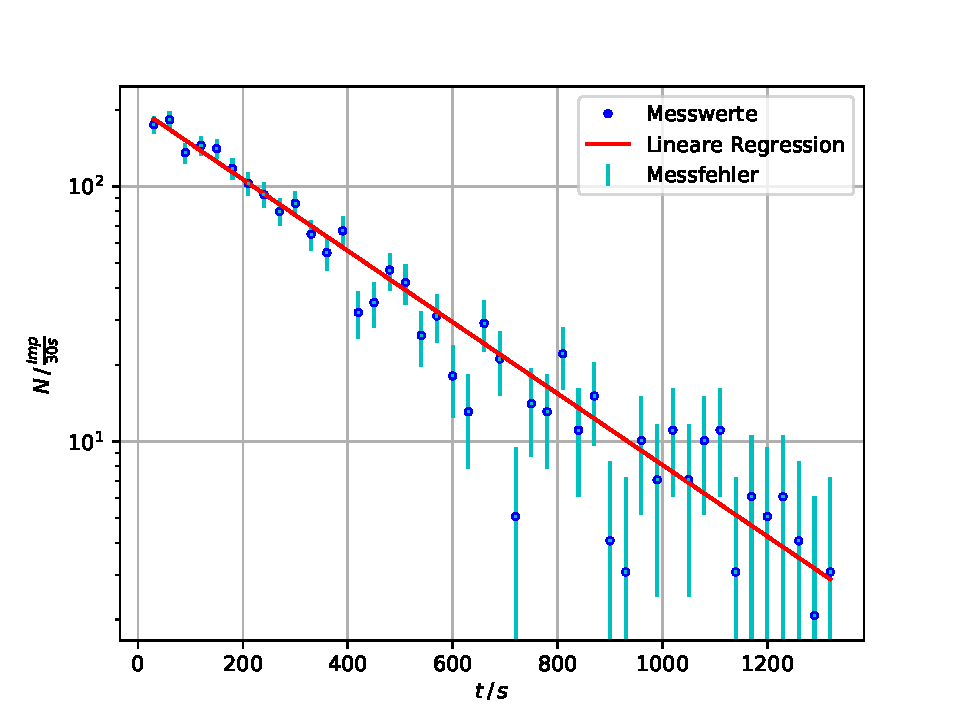
\includegraphics[width=0.8\textwidth]{content/data/vanadium.pdf}
    \caption{Die gemessenen Impulse $N_V$ (Vanadium) mit zugehörigem Fehler in Abhängigkeit von der Zeit $t$ in einem halblogarithmischen Diagramm dargestellt. Zu den Messwerten wird eine lineare Ausgleichsrechnung durchgeführt. \cite{matplotlib} \cite{numpy} \cite{scipy} \cite{uncertainties}}
    \label{fig:vanadium_plot}
\end{figure}
Aus dem $\lambda$ folgt sofort die Halbwertszeit \eqref{eqn:Halbwertszeit}
\begin{equation}
    T = \SI{215+-7}{\second}
\end{equation}
für Vanadium.
Eine weitere lineare Ausgleichsrechnung mit Werten bis zur doppelten Halbwertszeit ergibt keine genaueren Ergebnisse.

%Rhodium
\subsection{Bestimmung der Halbwertszeit von Rhodium}
Die Messintervalle für die Rhodiumprobe betragen $\Delta t = \SI{15}{\second}$.
Der Messfehler der Impulsrate der Rhodiumprobe $N_{Rh}$ wird nach $\Delta N_{Rh} = \sqrt{N_{Rh}}$ berechnet.
Die Untergrundrate angepasst an das Zeitintervall beträgt
\begin{equation*}
    N_U = \SI{6.96+-0.20}{\frac{Imp}{15 \second}} \, .
\end{equation*}
Diese wird von den gemessenen Impulsen der Rhodiumprobe $N_{Rh}$ subtrahiert und als $N_{dif}$ bezeichnet.
Die gemessenen Werte und die angepassten Messwerte befinden sich in Tab. \ref{tab:rhodium}.
\begin{table}
    \centering
    \begin{tabular}{ccc|}
    \toprule
    $t \,/\, \si{\second}$ & $N_{Rh} \,/\, \si{\frac{Imp}{15 \second}}$ & $N_{dif} \,/\, \si{\frac{Imp}{15 \second}}$ \\
    \midrule
    15 & 667  & $\SI{660+-26}{}$ \\
    30 & 585  & $\SI{578+-24}{}$ \\	 
    45 & 474  & $\SI{467+-22}{}$ \\
    60 & 399  & $\SI{392+-20}{}$ \\
    75 & 304  & $\SI{297+-17}{}$ \\
    90 & 253  & $\SI{246+-16}{}$ \\
    105 & 213 & $\SI{206+-15}{}$ \\
    120 & 173 & $\SI{166+-13}{}$ \\
    135 & 152 & $\SI{145+-12}{}$ \\
    150 & 126 & $\SI{119+-11}{}$ \\
    165 & 111 & $\SI{104+-11}{}$ \\
    180 & 92  & $\SI{85+-10}{}$ \\
    195 & 79  & $\SI{72+-9}{}$ \\
    210 & 74  & $\SI{67+-9}{}$ \\
    225 & 60  & $\SI{53+-8}{}$ \\
    240 & 52  & $\SI{45+-7}{}$ \\
    255 & 56  & $\SI{49+-7}{}$ \\
    270 & 53  & $\SI{46+-7}{}$ \\
    285 & 41  & $\SI{34+-6}{}$ \\
    300 & 36  & $\SI{29+-6}{}$ \\
    315 & 37  & $\SI{30+-6}{}$ \\
    330 & 32  & $\SI{25+-6}{}$ \\
    \bottomrule
    \end{tabular}
    \begin{tabular}{|ccc}
    \toprule
    $t \,/\, \si{\second}$ & $N_{Rh} \,/\, \si{\frac{Imp}{15 \second}}$ & $N_{dif} \,/\, \si{\frac{Imp}{15 \second}}$ \\
    \midrule
    345 & 36 & $\SI{29+-6}{}$ \\
    360 & 38 & $\SI{31+-6}{}$ \\
    375 & 34 & $\SI{27+-6}{}$ \\
    390 & 40 & $\SI{33+-6}{}$ \\
    405 & 21 & $\SI{14+-5}{}$ \\
    420 & 35 & $\SI{28+-6}{}$ \\
    435 & 33 & $\SI{26+-6}{}$ \\
    450 & 36 & $\SI{29+-6}{}$ \\
    465 & 20 & $\SI{13+-4}{}$ \\
    480 & 24 & $\SI{17+-5}{}$ \\
    495 & 30 & $\SI{23+-5}{}$ \\
    510 & 30 & $\SI{23+-5}{}$ \\
    525 & 26 & $\SI{19+-5}{}$ \\
    540 & 28 & $\SI{21+-5}{}$ \\
    555 & 23 & $\SI{16+-5}{}$ \\
    570 & 20 & $\SI{13+-4}{}$ \\
    585 & 28 & $\SI{21+-5}{}$ \\
    600 & 17 & $\SI{10+-4}{}$ \\
    615 & 26 & $\SI{19+-5}{}$ \\
    630 & 19 & $\SI{12+-4}{}$ \\
    645 & 13 & $\SI{6+-4}{}$ \\
    660 & 17 & $\SI{10+-4}{}$ \\
    \bottomrule
    \end{tabular}
    \caption{Zerfallsrate von Rhodium gemessen in einem Zeitintervall von $\SI{15}{\second}$.}
    \label{tab:rhodium}
\end{table}
Ab $t = \SI{270}{\second}$ ist nur der langsame Zerfall zu beobachten (siehe Abb. \ref{fig:rhodium_plot}).
Eine lineare Ausgleichsrechnung für den langsamen Zerfall ($t \geq \SI{270}{\second}$)
\begin{equation}
    \ln N_{dif} = -\lambda \cdot t + b
    \label{eqn:ausgleichsgerade}
\end{equation}
ergibt folgende Parameter:
\begin{align*}
    \lambda_\text{slow} = \SI{0.0027+-0.0004}{\frac{1}{\second}} \\
    b_\text{slow} = \SI{4.35+-0.17}{}
\end{align*}
Die Halbwertszeit \eqref{eqn:Halbwertszeit} für den langsamen Zerfall beträgt
\begin{equation*}
    T_\text{slow} = \SI{257+-37}{\second} \, .
\end{equation*}
Zur Bestimmung des schnellen Zerfalls wird $t \leq \SI{210}{\second}$ betrachtet.
Zuerst muss der langsame Zerfall von den Messwerten ($t \leq \SI{210}{\second}$) abgezogen werden
\begin{equation}
    N_\text{fast}(t) = N_{dif}(t) - (-\lambda_\text{slow} \cdot t + b_\text{slow})  \, . 
\end{equation}
Der langsame Zerfall wird durch die Geradengleichung mit den berechneten Parametern $\lambda_\text{slow}, b_\text{slow}$ beschrieben.
Die korrigierten Messwerte $N_\text{fast}$ mit zugehörigem Fehler sind in Abb. \ref{fig:rhodium_plot} eingezeichnet.
Eine Ausgleichsrechnung (siehe \eqref{eqn:ausgleichsgerade}) für den schnellen Zerfall ($t \leq \SI{210}{\second}$) mit den korrigierten Messwerten $N_\text{fast}$ ergibt folgende Parameter:
\begin{align*}
    \lambda_\text{fast} = \SI{0.0161+-0.0004}{\frac{1}{\second}} \\
    b = \SI{6.678+-0.025}{}
\end{align*}
Nach \eqref{eqn:Halbwertszeit} folgt aus $\lambda_\text{fast}$ die Halbwertszeit für den schnellen Zerfall
\begin{equation*}
    T_\text{fast} = \SI{43.0+-1.1}{\second} \, .
\end{equation*}
Die Ausgleichsgeraden, die Messwerte, sowieso die zugehörigen Fehler sind in einem halblogarithmischen Diagramm in Abb. \ref{fig:rhodium_plot} dargestellt.
\begin{figure}
    \centering
    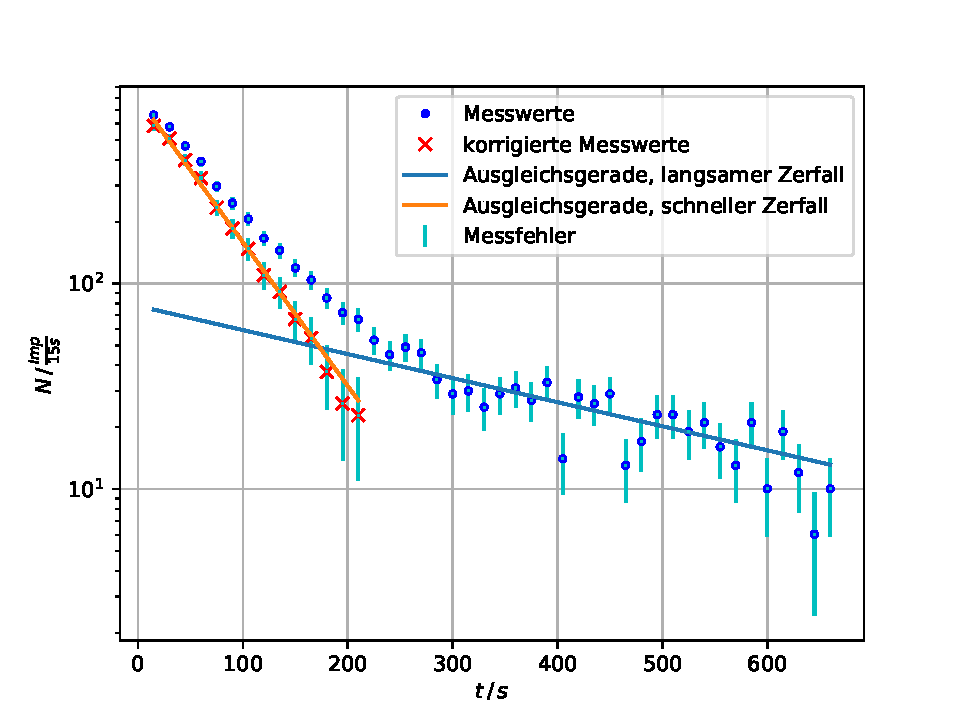
\includegraphics[width=0.8\textwidth]{content/data/rhodium.pdf}
    \caption{Die gemessenen Impulse $N_{Rh}$ (Rhodium) mit zugehörigem Fehler in Abhängigkeit von der Zeit $t$ in einem halblogarithmischen Diagramm dargestellt. Zudem wird eine lineare Ausgleichsrechnung für den langsamen und eine für den schnellen Zerfall durchgeführt. \cite{matplotlib} \cite{numpy} \cite{scipy} \cite{uncertainties}}
    \label{fig:rhodium_plot}
\end{figure}